% !TEX root = Projektdokumentation.tex

 \section{Kostenvoranschlag}
 Das Projekt läuft im Rahmen der Studienarbeit. Diese sieht einen Personenaufwand von 240 Stunden pro Person vor, was bei einer 2-Personen-Gruppe einen Aufwand von 480 Stunden macht. 
 Der Projektrahmen ist das Herbstsemester 2016, welches vom 19.09 - 23.12.2016 dauert und somit 14 Wochen umfasst. Es ist damit ein durchschnittlicher Wochenaufwand von 17 Stunden pro Person vorgesehen. 
 \section{Zeitliche Planung}
 \subsection{Phasen / Iterationen}
 Das Projekt ist in die Phasen Inception, Elaboration, Construction und Transition aufgeteilt. Die Inception-Phase hat bereits in der Woche vor dem Semesterbeginn stattgefunden. Die restlichen Phasen sind, wie in der Grafik auf der nächsten Seite ersichtlich, über das Herbstsemesters 2017 verteilt.
 
 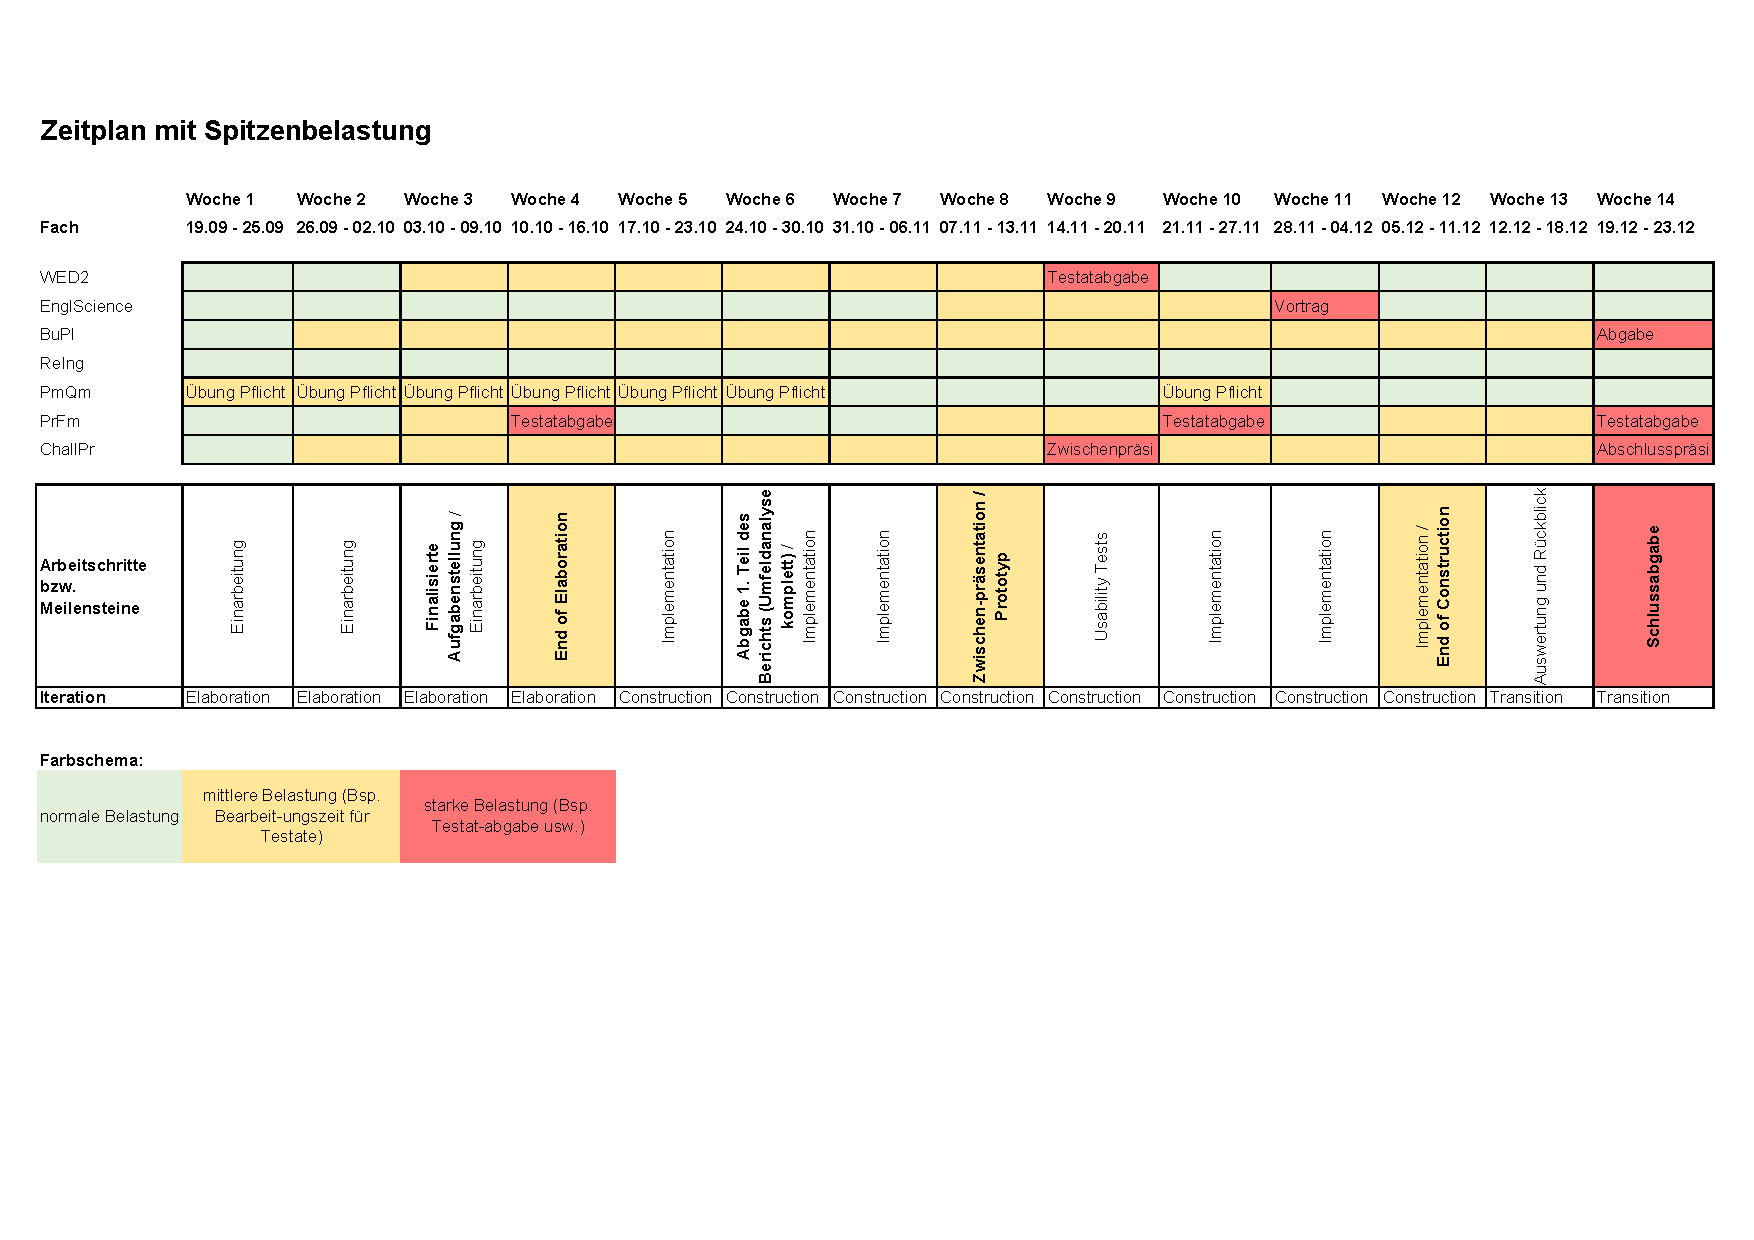
\includepdf[landscape=true]{Zeitplan_Spitzenbelastung.pdf}
 
 \subsection{Meilensteine}
 %ToDo: Beschreibungen der Meilensteine ergänzen
 \begin{tabularx}{\linewidth}{|X|c|X|}
 	\hline
 	\textbf{Meilenstein} & \textbf{Datum} & \textbf{Beschreibung} \\
 	\hline
 	Finalisierte Aufgabenstellung & 09.10.2016 & -- \\
 	\hline
 	End of Elaboration & 16.10.2016 & -- \\
 	\hline
 	Erster Teil des Berichts komplett & 30.10.2016 & Die Umfeldanalyse soll bereits komplett erstellt sein, damit Herr Heinzmann gegenlesen kann. \\
 	\hline
 	Zwischenpräsentation & 13.11.2016 & -- \\
 	\hline
 	Erster Prototyp & 13.11.2016 & -- \\
 	\hline
 	End of Construction & 11.12.2016 & -- \\
 	\hline
 	Schlussabgabe & 23.12.2016 & -- \\
 	\hline
 \end{tabularx}
 
 
 \todo{Die Meilensteine sollen konkret und messbar dargestellt werden.}
 \todo{Redmine Gantt-Diagramm hineinnehmen}